\documentclass[12pt]{article}

\usepackage{tikz}
\usetikzlibrary{automata}

\usepackage[a4paper,width=135mm,top=25mm,bottom=25mm]{geometry}

\usepackage{amsmath}

\usepackage[T1]{fontenc}

\usepackage{amssymb}

\usepackage{mathtools}
\DeclarePairedDelimiter\floor{\lfloor}{\rfloor}

\usepackage{fancyhdr}
\pagestyle{fancy}
\fancyhead{}
\fancyhead[RO]{Zadania Viktar Zhdanovich}
\fancyfoot{}
\fancyfoot[RO]{\textbf{\thepage}}
\fancyfoot[CO]{Zadania Viktar Zhdanovich}
\renewcommand{\headrulewidth}{0.4pt}
\renewcommand{\footrulewidth}{0.4pt}

\begin{document}

\begin{titlepage}
	\begin{center}
		{\LARGE\bfseries WSTĘP DO TEORII 			OBLICZALNOŚCI\par}
		\vspace{3cm}
		ZADANIA DLA CHĘTNYCH \par
		Zestaw 1. Wersja 1.0.0 \par
	\end{center}
	\vfill\centering VIKTAR ZHDANOVICH LB6 \par
\end{titlepage}

\newpage

\noindent\textbf{Zad 1.1.} Zaprojektuj  maszynę  Turinga,  która  oblicza  funkcję  odejmowania ograniczonego \textit{f} dla liczb naturalnych \textit{m} i \textit{n} w reprezentacji unarnej, czyli
\[ f(m,n) = m - n = 
  \begin{cases}
   	m - n, & \text{jeżeli } m \geq n, \\
   	0, & \text{jezeli } m < n
  \end{cases}
\]
Narysuj diagram przejść. Dla zaprojektowanej maszyny wykonaj dwa obliczenia (wykonaj rysunki taśmy i zapisz konfiguracje).

 Rozwiązanie.
 
\[M=(Q,\Gamma,\Sigma,\delta,q_0,\bigtriangledown,F)=(\{q_0,q_1,q_2,q_3,q_4,q_5,q_6,q_7\},\{1,0\},\{1,0,\bigtriangledown\},\delta,q_0,\bigtriangledown,\{q_7\}).\]

\vspace{20pt}

\begin{center}
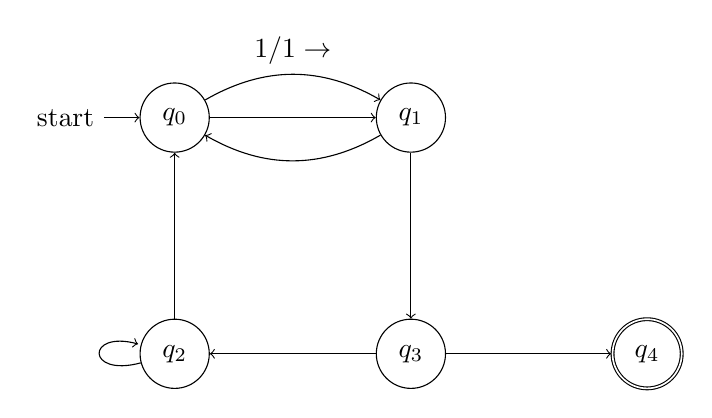
\begin{tikzpicture}[->,node distance=3cm,auto]

\node[initial,state](A){$q_0$};
\node[state](B)[right of=A]{$q_1$};
\node[state](C)[below of=A]{$q_2$};
\node[state](D)[below of=B]{$q_3$};
\node[state,accepting](E)[right of=D]{$q_4$};

\path(A)edge[bend left]node{$1/1\rightarrow$}(B)
	edge(B)
	(B)edge[bend left](A)
	edge(D)
	(C)edge(A)
	edge[loop left](C)
	(D)edge(C)
	edge(E);

\end{tikzpicture}
\end{center}

\newpage
\noindent\textbf{Zad 1.2.} Zaprojektuj maszynę Turinga, która oblicza funkcję mnożenia \textit{f} dla liczb naturalnych \textit{m} i \textit{n} w reprezentacji unarnej, czyli
\[f(m,n)=m \cdot n\]
Narysuj diagram przejść. Dla zaprojektowanej maszyny wykonaj dwa obliczenia, w tym pomnóż 3·2 lub 2·3 (wykonaj rysunki taśmy i zapisz konfiguracje).

 Rozwiązanie.
 
\[M=(Q,\Gamma,\Sigma,\delta,q_0,\bigtriangledown,F)=(\{q_0, ... ,q_{11}\},\{1,0\},\{1,0,\bigtriangledown\},\delta,q_0,\bigtriangledown,\{q_{11}\}).\]

\newpage

\noindent\textbf{Zad 1.3.} Zaprojektuj  maszynę  Turinga,  która  oblicza  funkcję \textit{f} dla  liczbynaturalnej \textit{n} w reprezentacji unarnej, gdzie
\[f(n)=
	\begin{cases}
	\frac{n}{2}, & \text{jeżeli \textit{n} jest parzysta,} \\
   	\frac{n+1}{2}, & \text{jezeli \textit{n} jest niparzysta.}
	\end{cases}	
\]
Narysuj diagram przejść. Dla zaprojektowanej maszyny wykonaj dwa obliczenia (wykonaj rysunki taśmy i zapisz konfiguracje).

 Rozwiązanie.
 
\[M=(Q,\Gamma,\Sigma,\delta,q_0,\bigtriangledown,F)=(\{q_0,...,q_9\},\{1\},\{1,\bigtriangledown\},\delta,q_0,\bigtriangledown,\{q_9\}).\]

\newpage

\noindent\textbf{Zad 1.5.} Zaprojektuj  maszynę  Turinga,  która  oblicza  funkcję \textit{f} dla  liczby naturalnej \textit{n} w reprezentacji unarnej, gdzie
\[f(n)=\floor*{\frac{n}{2}}\]
Narysuj diagram przejść. Dla zaprojektowanej maszyny wykonaj dwa obliczenia (wykonaj rysunki taśmy i zapisz konfiguracje).

 Rozwiązanie.

\[M=(Q,\Gamma,\Sigma,\delta,q_0,\bigtriangledown,F)=(\{q_0,...,q_6\},\{1\},\{1,\bigtriangledown\},\delta,q_0,\bigtriangledown,\{q_6\}).\]

\newpage

\noindent\textbf{Zad 1.7.} Zaprojektuj maszynę Turinga, która oblicza funkcję signum (znaku)
\[sgn(n)=
	\begin{cases}
	1, & \text{jeżeli \textit{n} > 0,} \\
	0, & \text{jeżeli \textit{n} = 0}
	\end{cases}
\]
Narysuj diagram przejść. Dla zaprojektowanej maszyny wykonaj dwa obliczenia (wykonaj rysunki taśmy i zapisz konfiguracje).

 Rozwiązanie.
 
\[M=(Q,\Gamma,\Sigma,\delta,q_0,\bigtriangledown,F)=(\{q_0,q_1,q_2,q_3,q_4\},\{1\},\{1,\bigtriangledown\},\delta,q_0,\bigtriangledown,\{q_4\}).\]

\newpage

\noindent\textbf{Zad 1.9.} Zaprojektuj maszynę Turinga, która oblicza funkcję
\[f(n)=
	\begin{cases}
	0, & \text{jeżeli \textit{n} jest parzysta,} \\
	1, & \text{jeżeli \textit{n} jest nieparzysta.}
	\end{cases}
\]
Narysuj diagram przejść. Dla zaprojektowanej maszyny wykonaj dwa obliczenia (wykonaj rysunki taśmy i zapisz konfiguracje).

 Rozwiązanie.

\[M=(Q,\Gamma,\Sigma,\delta,q_0,\bigtriangledown,F)=(\{q_0,q_1,q_2,q_3,q_4,q_5\},\{1\},\{1,\bigtriangledown\},\delta,q_0,\bigtriangledown,\{q_5\}).\]

\newpage

\noindent\textbf{Zad 1.11.} Zaprojektuj maszynę Turinga, która oblicza funkcję maksimum dla liczb naturalnych \textit{m} i \textit{n} w reprezentacji unarnej, czyli
\[f(n)=max(m,n).\]
Narysuj diagram przejść. Dla zaprojektowanej maszyny wykonaj dwa obliczenia (wykonaj rysunki taśmy i zapisz konfiguracje).

 Rozwiązanie.
 
\[M=(Q,\Gamma,\Sigma,\delta,q_0,\bigtriangledown,F)=(\{q_0,...,q_{12}\},\{1,0\},\{1,0,X,\bigtriangledown\},\delta,q_0,\bigtriangledown,\{q_{12}\}).\]

\newpage

\noindent\textbf{Zad 1.13.} Zaprojektuj maszynę Turinga, która oblicza funkcję
\[f(m,n)=n^2\]
dla liczby naturalnej \textit{n} w reprezentacji unarnej. Narysuj diagram przejść. Dla zaprojektowanej maszyny wykonaj dwa obliczenia (wykonaj rysunki taśmy i zapisz konfiguracje).

 Rozwiązanie.
 
\[M=(Q,\Gamma,\Sigma,\delta,q_0,\bigtriangledown,F)=(\{q_0,...,q_{17}\},\{1,0\},\{1,0,X,Y,r,\bigtriangledown\},\delta,q_0,\bigtriangledown,\{q_{17}\}).\]

\newpage

\noindent\textbf{Zad 1.19.} Zaprojektuj maszynę Turinga, która kopiuje wejściowy łańcuch \textit{w} dla alfabetu $\Sigma=\{a,b\}$. Rozwiązanie może nie zawierać separatora
\[q_0w \overset{*}{\vdash} q_fww\]
lub  może  zawierać  dowolny  separator,  na  przykład  separatorem  może  być blank, czyli
\[q_0w \overset{*}{\vdash} q_fw \bigtriangledown w.\]
Narysuj diagram przejść. Dla zaprojektowanej maszyny wykonaj dwa obliczenia (wykonaj rysunki taśmy i zapisz konfiguracje).

 Rozwiązanie.
 
\[M=(Q,\Gamma,\Sigma,\delta,q_0,\bigtriangledown,F)=(\{q_0,...,q_{10}\},\{a,b\},\{a,b,s,X,Y,\bigtriangledown\},\delta,q_0,\bigtriangledown,\{q_{10}\}).\]

\newpage

\noindent\textbf{Zad 1.22.} Zaprojektuj  maszynę  Turinga  nad  alfabetem $\Sigma=\{a,b\}$,  która akceptuje język
\[L=\{\text{\textit{w}: \textit{w} zawiera  równą liczbę symboli \textit{a} i \textit{b}}\}.\]
Narysuj diagram przejść. Dla zaprojektowanej maszyny wykonaj dwa obliczenia (wykonaj rysunki taśmy i zapisz konfiguracje).

 Rozwiązanie.
 
\[M=(Q,\Gamma,\Sigma,\delta,q_0,\bigtriangledown,F)=(\{q_0,...,q_6\},\{a,b\},\{a,b,X,Y,\bigtriangledown\},\delta,q_0,\bigtriangledown,\{q_6\}).\]

\newpage

\noindent\textbf{Zad 1.23.} Zaprojektuj maszynę Turinga, która akceptuje język
\[L=\{\text{\textit{w}: |\textit{w}| jest parzysta}\}\]
nad alfabetem $\Sigma=\{0,1\}$. Narysuj diagram przejść. Dla zaprojektowanej maszyny wykonaj dwa obliczenia (wykonaj rysunki taśmy i zapisz konfiguracje).

 Rozwiązanie.
 
\[M=(Q,\Gamma,\Sigma,\delta,q_0,\bigtriangledown,F)=(\{q_0,q_1,q_2\},\{1,0\},\{1,0,\bigtriangledown\},\delta,q_0,\bigtriangledown,\{q_2\}).\]

\newpage

\noindent\textbf{Zad 1.25.} Niech $\Sigma=\{a,b\}$. Zaprojektuj maszynę Turinga, która akceptuje język
\[L=\{\text{\textit{w}${\textit{w}^\textit{R}}$: \textit{w} $\in$ $\{a,b\}^*$\},}\]
gdzie ${\textit{w}^\textit{R}}$ oznacza \textbf{odwrócenie} \textit{w},  a  więc  jeśli \textit{w} = $a_1a_2...a_k$, to ${\textit{w}^\textit{R}}$ = $a_ka_{k-1}...a_1$. Narysuj  diagram  przejść. Dla  zaprojektowanej  maszyny  wykonaj dwa obliczenia (wykonaj rysunki taśmy i zapisz konfiguracje).

 Rozwiązanie.
 
\[M=(Q,\Gamma,\Sigma,\delta,q_0,\bigtriangledown,F)=(\{q_0,...,q_8\},\{a,b\},\{a,b,X,Y,\bigtriangledown\},\delta,q_0,\bigtriangledown,\{q_8\}).\]

\newpage

\noindent\textbf{Zad 1.27.} Niech $\Sigma=\{0,1\}$.  Zaprojektuj  maszynę  Turinga,  która  oblicza odwrócenie łańcucha, czyli funkcję
\[f(w)=w^R\]
gdzie $\textit{w}\in\{0,1\}^+$ oraz ${\textit{w}^\textit{R}}$ oznacza \textbf{odwrócenie} \textit{w},  a  więc  jeśli \textit{w} = $a_1a_2...a_k$, to ${\textit{w}^\textit{R}}$ = $a_ka_{k-1}...a_1$. Narysuj  diagram  przejść. Dla  zaprojektowanej  maszyny  wykonaj dwa obliczenia (wykonaj rysunki taśmy i zapisz konfiguracje).

 Rozwiązanie.
 
\[M=(Q,\Gamma,\Sigma,\delta,q_0,\bigtriangledown,F)=(\{q_0,...,q_9\},\{1,0\},\{1,0,s,X,Y,\bigtriangledown\},\delta,q_0,\bigtriangledown,\{q_9\}).\]

\newpage

\noindent\textbf{Zad 1.30.} Zaprojektuj maszynę Turinga, która akceptuje język
\[L=\{\text{$x^ny^n$: \textit{n} $\geq$ 1}\}\]
nad alfabetem $\Sigma=\{x,y\}$. Narysuj diagram przejść. Dla zaprojektowanej maszyny wykonaj dwa obliczenia (wykonaj rysunki taśmy i zapisz konfiguracje).

 Rozwiązanie.
 
\[M=(Q,\Gamma,\Sigma,\delta,q_0,\bigtriangledown,F)=(\{q_0,...,q_8\},\{x,y\},\{x,y,A,B,\bigtriangledown\},\delta,q_0,\bigtriangledown,\{q_8\}).\]

\newpage

\noindent\textbf{Zad 1.46.} Wypisz cztery przykładowe łańcuchy opisywane przez wyrażenie \textbf{a}$(\textbf{a}+\textbf{b})^*$\textbf{bb}. Czy można skonstruować (deterministyczną) maszynę Turinga,która akceptuje język
\[L=L(\textbf{a}(\textbf{a}+\textbf{b})^*\textbf{bb})?\]
Jeżeli można, to narysuj diagram przejść i dla zaprojektowanej maszyny wykonaj dwa obliczenia (wykonaj rysunki taśmy i zapisz konfiguracje).

 Rozwiązanie.
 
\[M=(Q,\Gamma,\Sigma,\delta,q_0,\bigtriangledown,F)=(\{q_0,q_1,q_2,q_3,q_4\},\{a,b\},\{a,b,\bigtriangledown\},\delta,q_0,\bigtriangledown,\{q_4\}).\]

\newpage

\noindent\textbf{Zad 1.47.} Wypisz cztery przykładowe łańcuchy opisywane przez wyrażenie \textbf{10+(0+11)$\textbf{0}^*$1}. Czy można skonstruować (deterministyczną) maszynę Turinga, która akceptuje język
\[L=L(\textbf{10+(0+11)$\textbf{0}^*$1})?\]
Jeżeli można, to narysuj diagram przejść i dla zaprojektowanej maszyny wy-konaj dwa obliczenia (wykonaj rysunki taśmy i zapisz konfiguracje).

 Rozwiązanie.
 
\[M=(Q,\Gamma,\Sigma,\delta,q_0,\bigtriangledown,F)=(\{q_0,...,q_8\},\{1,0\},\{1,0,\bigtriangledown\},\delta,q_0,\bigtriangledown,\{q_8\}).\]

\newpage

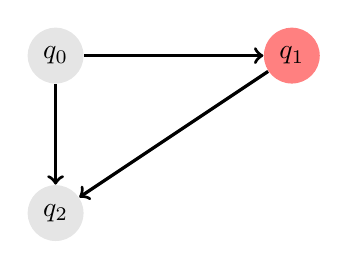
\begin{tikzpicture}

\tikzstyle{vertex}=[circle,fill=black!10]
\tikzstyle{selected vertex}=[vertex,fill=red!50]
\tikzstyle{edge}=[->,very thick]

\node[vertex](v1)at(0,0){$q_0$};
\node[selected vertex](v2)at(3,0){$q_1$}; % 3cm
\node[vertex](v3)at(0,-2){$q_2$};

\draw[edge](v1)--(v2);
\draw[edge](v1)--(v3);
\draw[edge](v2)--(v3);

\end{tikzpicture}

\vspace{40pt}

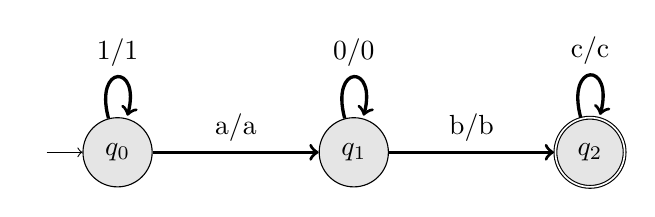
\begin{tikzpicture}[->,node distance=3cm,auto]

\tikzstyle{vertex}=[circle,fill=black!10]
\tikzstyle{edge}=[->,very thick]

\node[state,
	vertex,
	initial,
 	initial text=
 	](A){$q_0$};
 	
\node[state,vertex](B)[right of=A]{$q_1$};

\node[state,vertex,accepting](C)[right of=B]{$q_2$};

\path[edge](A)edge[loop above]node{1/1}(A)
	edge node{a/a}(B)
	(B)edge[loop above]node{0/0}(B)
	edge node{b/b}(C)
	(C)edge[loop above]node{c/c}(C);

\end{tikzpicture}

\vspace{40pt}

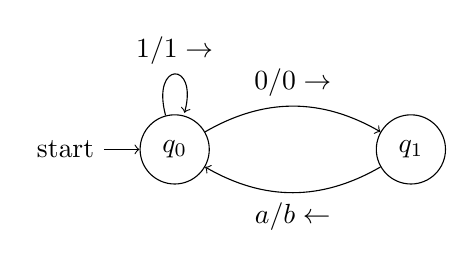
\begin{tikzpicture}[->,node distance=3cm,auto]

\node[initial,state](A){$q_0$};
\node[state](B)[right of=A]{$q_1$};

\path(A)edge[loop above]node{$1/1\rightarrow$}(A)
	edge[bend left]node{$0/0\rightarrow$}(B)
	(B)edge[bend left]node{$a/b\leftarrow$}(A);

\end{tikzpicture}

\vspace{40pt}

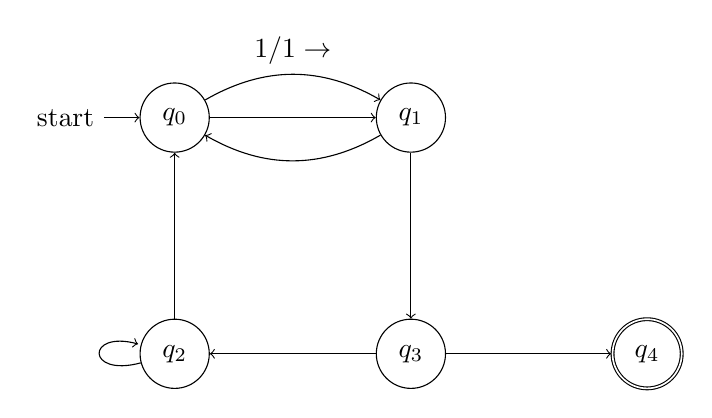
\begin{tikzpicture}[->,node distance=3cm,auto]

\node[initial,state](A){$q_0$};
\node[state](B)[right of=A]{$q_1$};
\node[state](C)[below of=A]{$q_2$};
\node[state](D)[below of=B]{$q_3$};
\node[state,accepting](E)[right of=D]{$q_4$};

\path(A)edge[bend left]node{$1/1\rightarrow$}(B)
	edge(B)
	(B)edge[bend left](A)
	edge(D)
	(C)edge(A)
	edge[loop left](C)
	(D)edge(C)
	edge(E);

\end{tikzpicture}

\end{document}